\documentclass[11pt,a4paper]{article}

% ── Packages ──
\usepackage[utf8]{inputenc}
\usepackage[T1]{fontenc}
\usepackage{lmodern}
\usepackage[margin=2.5cm]{geometry}
\usepackage{graphicx}
\usepackage{xcolor}
\usepackage{hyperref}
\usepackage{listings}
\usepackage{booktabs}
\usepackage{tabularx}
\usepackage{longtable}
\usepackage{fancyhdr}
\usepackage{titlesec}
\usepackage{enumitem}
\usepackage{tcolorbox}
\usepackage{float}
\usepackage{caption}
\usepackage{microtype}
\usepackage{parskip}
\usepackage{tikz}
\usetikzlibrary{shapes.geometric, arrows.meta, positioning, calc}

% ── Colors ──
\definecolor{mpblue}{HTML}{2563EB}
\definecolor{mpnavy}{HTML}{0F172A}
\definecolor{mpslate}{HTML}{1E293B}
\definecolor{mpcritical}{HTML}{EF4444}
\definecolor{mpwarning}{HTML}{EAB308}
\definecolor{mpgreen}{HTML}{22C55E}
\definecolor{codebg}{HTML}{F1F5F9}
\definecolor{codeframe}{HTML}{CBD5E1}
\definecolor{linkblue}{HTML}{3B82F6}

% ── Hyperref config ──
\hypersetup{
  colorlinks=true,
  linkcolor=mpblue,
  urlcolor=linkblue,
  citecolor=mpblue,
  pdfauthor={Micke Samuel},
  pdftitle={MigrationPilot v1.1.0 — Product Report},
  pdfsubject={PostgreSQL Migration Safety CLI},
}

% ── Code listings ──
\lstdefinestyle{terminal}{
  backgroundcolor=\color{codebg},
  basicstyle=\ttfamily\small,
  breaklines=true,
  breakatwhitespace=false,
  frame=single,
  rulecolor=\color{codeframe},
  framesep=6pt,
  xleftmargin=6pt,
  xrightmargin=6pt,
  aboveskip=10pt,
  belowskip=10pt,
  columns=fullflexible,
  keepspaces=true,
  showstringspaces=false,
  literate={✗}{{\textcolor{mpcritical}{\texttimes}}}1
           {⚠}{{\textcolor{mpwarning}{!}}}1
           {✓}{{\textcolor{mpgreen}{\checkmark}}}1
           {█}{{\textcolor{mpgreen}{\rule{6pt}{8pt}}}}1
           {░}{{\textcolor{codebg}{\rule{6pt}{8pt}}}}1
           {─}{-}1
           {╔}{+}1 {╗}{+}1 {╚}{+}1 {╝}{+}1
           {║}{|}1 {═}{=}1
           {┌}{+}1 {┐}{+}1 {└}{+}1 {┘}{+}1
           {│}{|}1 {├}{+}1 {┤}{+}1
           {┬}{+}1 {┴}{+}1 {┼}{+}1
           {◷}{{hours}}5
           {⚡}{{instant}}7
}

\lstdefinestyle{sql}{
  backgroundcolor=\color{codebg},
  basicstyle=\ttfamily\small,
  breaklines=true,
  frame=single,
  rulecolor=\color{codeframe},
  framesep=6pt,
  xleftmargin=6pt,
  xrightmargin=6pt,
  language=SQL,
  keywordstyle=\color{mpblue}\bfseries,
  commentstyle=\color{gray},
  stringstyle=\color{mpgreen!70!black},
  columns=fullflexible,
  keepspaces=true,
  morekeywords={CONCURRENTLY,VACUUM,REINDEX,CLUSTER},
}

\lstdefinestyle{yaml}{
  backgroundcolor=\color{codebg},
  basicstyle=\ttfamily\small,
  breaklines=true,
  frame=single,
  rulecolor=\color{codeframe},
  framesep=6pt,
  xleftmargin=6pt,
  xrightmargin=6pt,
  columns=fullflexible,
  keepspaces=true,
}

\lstdefinestyle{json}{
  backgroundcolor=\color{codebg},
  basicstyle=\ttfamily\footnotesize,
  breaklines=true,
  frame=single,
  rulecolor=\color{codeframe},
  framesep=6pt,
  xleftmargin=6pt,
  xrightmargin=6pt,
  columns=fullflexible,
  keepspaces=true,
}

% ── Header/Footer ──
\pagestyle{fancy}
\fancyhf{}
\fancyhead[L]{\small\textcolor{gray}{MigrationPilot v1.1.0}}
\fancyhead[R]{\small\textcolor{gray}{Product Report}}
\fancyfoot[C]{\small\textcolor{gray}{\thepage}}
\renewcommand{\headrulewidth}{0.4pt}
\renewcommand{\footrulewidth}{0pt}

% ── Section styling ──
\titleformat{\section}{\Large\bfseries\color{mpblue}}{}{0em}{}[\vspace{-4pt}\textcolor{mpblue}{\rule{\textwidth}{1pt}}]
\titleformat{\subsection}{\large\bfseries}{}{0em}{}
\titleformat{\subsubsection}{\normalsize\bfseries}{}{0em}{}

% ── Colored boxes ──
\tcbuselibrary{skins,breakable}

\newtcolorbox{criticalbox}{
  colback=mpcritical!5,
  colframe=mpcritical!60,
  fonttitle=\bfseries,
  title=CRITICAL,
  sharp corners,
  boxrule=0.5pt,
  left=6pt, right=6pt, top=4pt, bottom=4pt,
}

\newtcolorbox{warningbox}{
  colback=mpwarning!5,
  colframe=mpwarning!60,
  fonttitle=\bfseries,
  title=WARNING,
  sharp corners,
  boxrule=0.5pt,
  left=6pt, right=6pt, top=4pt, bottom=4pt,
}

\newtcolorbox{greenbox}{
  colback=mpgreen!5,
  colframe=mpgreen!60,
  fonttitle=\bfseries,
  title=SAFE,
  sharp corners,
  boxrule=0.5pt,
  left=6pt, right=6pt, top=4pt, bottom=4pt,
}

\newtcolorbox{infobox}{
  colback=mpblue!5,
  colframe=mpblue!60,
  sharp corners,
  boxrule=0.5pt,
  left=6pt, right=6pt, top=4pt, bottom=4pt,
}

% ── Document ──
\begin{document}

% ══════════════════════════════════════════════════════════
% TITLE PAGE
% ══════════════════════════════════════════════════════════

\begin{titlepage}
\begin{center}
\vspace*{2cm}

% Logo

\begin{tikzpicture}
  \node[fill=mpblue, rounded corners=8pt, minimum width=2cm, minimum height=2cm, text=white, font=\Huge\bfseries] {MP};
\end{tikzpicture}

\vspace{1cm}

{\Huge\bfseries MigrationPilot}\\[0.3cm]
{\Large\color{gray} Product Report \& User Experience Walkthrough}

\vspace{1.5cm}

{\large Version 1.1.0}\\[0.3cm]
{\color{gray} February 2026}

\vspace{2cm}

\begin{tcolorbox}[colback=mpblue!5, colframe=mpblue!40, width=12cm, center, sharp corners]
\centering
\textbf{Know exactly what your PostgreSQL migration\\will do to production --- before you merge.}\\[0.5cm]
48 safety rules $\cdot$ Auto-fix $\cdot$ Risk scoring $\cdot$ GitHub Action\\
6 output formats $\cdot$ 14 framework detection $\cdot$ Watch mode
\end{tcolorbox}

\vfill

{\color{gray}
\textbf{Author:} Micke Samuel\\
\textbf{Website:} \url{https://migrationpilot.dev}\\
\textbf{Repository:} \url{https://github.com/mickelsamuel/migrationpilot}\\
\textbf{License:} MIT
}

\end{center}
\end{titlepage}

% ══════════════════════════════════════════════════════════
% TABLE OF CONTENTS
% ══════════════════════════════════════════════════════════

\tableofcontents
\newpage

% ══════════════════════════════════════════════════════════
% 1. EXECUTIVE SUMMARY
% ══════════════════════════════════════════════════════════

\section{Executive Summary}

MigrationPilot is a PostgreSQL migration safety tool that analyzes DDL (Data Definition Language) statements for dangerous patterns \textbf{before} they reach production. It works as a CLI, GitHub Action, and Node.js library.

\begin{infobox}
\textbf{Key Statistics:}
\begin{itemize}[nosep]
  \item \textbf{48 safety rules} (45 free, 3 Pro) --- more than any competitor
  \item \textbf{6 auto-fixable rules} with \texttt{--fix} flag
  \item \textbf{6 output formats:} text, JSON, SARIF v2.1.0, markdown, quiet, verbose
  \item \textbf{14 migration frameworks} auto-detected
  \item \textbf{550+ tests} across 31 test files
  \item \textbf{8 CLI commands:} analyze, check, plan, init, detect, watch, hook, list-rules
  \item \textbf{3 config presets:} recommended, strict, ci
  \item \textbf{Risk scoring:} RED / YELLOW / GREEN (0--100)
\end{itemize}
\end{infobox}

\subsection{Open-Core Business Model}

\begin{tabularx}{\textwidth}{lXl}
\toprule
\textbf{Tier} & \textbf{What's Included} & \textbf{Price} \\
\midrule
Free & 45 safety rules, CLI, GitHub Action, all output formats, auto-fix, PR comments, config, watch mode, hooks, framework detection & \$0 forever \\
Pro & Everything in Free + production context queries (pg\_stat\_*, pg\_class), 3 production rules (MP013/014/019), enhanced risk scoring & \$29/mo \\
Enterprise & Everything in Pro + team license management, SSO/SAML, audit logs, dedicated support, custom rules & Custom \\
\bottomrule
\end{tabularx}

\subsection{Competitive Position}

\begin{tabularx}{\textwidth}{lcccc}
\toprule
\textbf{Metric} & \textbf{MigrationPilot} & \textbf{Squawk} & \textbf{Atlas} \\
\midrule
Total rules & \textbf{48} & 31 & $\sim$15 \\
Free rules & \textbf{45} & 31 & 0 (paywalled) \\
Auto-fix & \textbf{6 rules} & 0 & 0 \\
Output formats & \textbf{6} & 3 & 2 \\
Framework detection & \textbf{14} & 0 & 0 \\
Watch mode & \textbf{Yes} & No & No \\
Config presets & \textbf{3} & 0 & 0 \\
Programmatic API & \textbf{Yes} & No & Yes (Go) \\
\bottomrule
\end{tabularx}

\newpage

% ══════════════════════════════════════════════════════════
% 2. WEBSITE WALKTHROUGH
% ══════════════════════════════════════════════════════════

\section{Website Walkthrough}

The MigrationPilot landing page is a single-page Next.js 16 application with Tailwind CSS 4, featuring a dark-themed design optimized for developer audiences. It is deployed at \url{https://migrationpilot.dev} and statically generated for performance.

\subsection{Hero Section}

The hero section communicates the core value proposition immediately: ``Know what your migration will do to production.'' The version badge (v1.1.0) and feature highlights (48 rules, auto-fix, risk scoring) establish credibility.

\begin{figure}[H]
\centering
\includegraphics[width=\textwidth]{site-hero.png}
\caption{Landing page hero section with version badge, headline, value proposition, and CTAs.}
\end{figure}

\textbf{Key elements:}
\begin{itemize}[nosep]
  \item Navigation bar: Features, Rules, Pricing, GitHub, Get Started CTA
  \item Version badge: ``v1.1.0 --- 48 rules, auto-fix, risk scoring''
  \item Two CTAs: ``Get Started Free'' (links to pricing) and ``View on GitHub''
  \item Clarifying note: ``45 rules free forever. Pro adds production context.''
\end{itemize}

\subsection{Interactive Demo Terminal}

Below the hero, an interactive terminal demo shows real CLI output --- a RED-risk migration with violations, safe alternatives, and timing.

\begin{figure}[H]
\centering
\includegraphics[width=\textwidth]{site-demo.png}
\caption{Simulated terminal showing analysis output with risk score, lock types, and violations.}
\end{figure}

\subsection{Features Grid}

Nine feature cards organized in a 3$\times$3 grid, each with an emoji icon, title, and description:

\begin{figure}[H]
\centering
\includegraphics[width=\textwidth]{site-features.png}
\caption{Feature grid: Lock Analysis, 48 Safety Rules, Auto-fix, Risk Scoring, GitHub Action, 14 Framework Detection, Watch Mode, Config + Presets, 6 Output Formats.}
\end{figure}

\subsection{Complete Rules Catalog}

All 48 rules displayed in four categories, each showing the rule ID, severity badge, name, and one-line description:

\begin{figure}[H]
\centering
\includegraphics[width=\textwidth]{site-rules.png}
\caption{Rules section showing Lock Safety rules (critical severity) and Data Safety rules. All 48 rules are listed.}
\end{figure}

\textbf{Rule categories:}
\begin{itemize}[nosep]
  \item \textbf{Lock Safety} (16 rules) --- Critical patterns that acquire dangerous locks
  \item \textbf{Data Safety} (3 rules) --- Irreversible data destruction
  \item \textbf{Best Practices} (26 rules) --- Schema design and migration hygiene
  \item \textbf{Production Context} (3 rules, Pro) --- Traffic and size-aware checks
\end{itemize}

\subsection{Pricing Section}

Three-tier pricing with transparent feature lists:

\begin{figure}[H]
\centering
\includegraphics[width=\textwidth]{site-pricing.png}
\caption{Pricing section: Free (\$0 forever), Pro (\$29/month), Enterprise (custom).}
\end{figure}

\subsection{CTA Section \& Footer}

The bottom CTA shows a GitHub Action YAML snippet for instant adoption. The footer has four columns (Product, Resources, Company) with comprehensive links.

\begin{figure}[H]
\centering
\includegraphics[width=\textwidth]{site-footer.png}
\caption{Bottom CTA with GitHub Action snippet and 4-column footer with ``Made in Montreal'' tag.}
\end{figure}

\subsection{Individual Rule Pages}

Each of the 48 rules has a dedicated page at \texttt{/rules/mp\{id\}} with full documentation:

\begin{figure}[H]
\centering
\includegraphics[width=0.95\textwidth]{site-rule-mp001.png}
\caption{Rule detail page for MP001 (require-concurrent-index-creation) showing severity badges, detection description, bad/good examples, auto-fix instructions, and configuration.}
\end{figure}

\begin{figure}[H]
\centering
\includegraphics[width=0.95\textwidth]{site-rule-mp013-pro.png}
\caption{Pro rule page for MP013 (high-traffic-table-ddl) showing the ``Pro'' tier badge.}
\end{figure}

\textbf{Each rule page includes:}
\begin{itemize}[nosep]
  \item Severity badge (CRITICAL/WARNING), auto-fixable badge, tier badge (Free/Pro)
  \item ``What It Detects'' description
  \item ``Why It's Dangerous'' explanation
  \item Bad Example (red-tinted SQL code block)
  \item Good Example (green-tinted SQL code block)
  \item Auto-fix instructions (if applicable)
  \item Configuration YAML snippet
  \item Links: back to all rules, view on GitHub
\end{itemize}

\newpage

% ══════════════════════════════════════════════════════════
% 3. CLI WALKTHROUGH
% ══════════════════════════════════════════════════════════

\section{CLI Walkthrough}

\subsection{Installation \& Version}

\begin{lstlisting}[style=terminal]
$ npm install -g migrationpilot

$ migrationpilot --version
1.1.0
node v24.13.0
platform win32-x64
rules: 48 (45 free, 3 pro)
\end{lstlisting}

The enriched version output shows the Node.js version, platform, and rule breakdown.

\subsection{Help \& Commands}

\begin{lstlisting}[style=terminal]
$ migrationpilot --help
Usage: migrationpilot [options] [command]

Know exactly what your PostgreSQL migration will do to
production -- before you merge.

Options:
  -V, --version             output the version number
  --no-color                Disable colored output
  -h, --help                display help for command

Commands:
  init                      Generate a .migrationpilotrc.yml config
  list-rules [options]      List all available safety rules
  detect [dir]              Auto-detect migration framework
  watch [options] <dir>     Watch migration files and re-analyze
  hook <action>             Install/uninstall git pre-commit hook
  plan [options] <file>     Show a visual execution plan
  analyze [options] [file]  Analyze a SQL migration file for safety
  check [options] <dir>     Check all migration files in a directory
  help [command]            display help for command
\end{lstlisting}

\subsection{Core Analysis --- Unsafe Migration}

Given an unsafe migration file:

\begin{lstlisting}[style=sql]
-- demo-unsafe.sql
CREATE INDEX idx_users_email ON users (email);
ALTER TABLE orders ADD COLUMN total numeric DEFAULT 0;
ALTER TABLE users ALTER COLUMN name TYPE varchar(50);
VACUUM FULL users;
DROP TABLE legacy_data;
\end{lstlisting}

Running \texttt{migrationpilot analyze demo-unsafe.sql} produces:

\begin{criticalbox}
\textbf{Risk: YELLOW --- Score: 40/100}\\
5 statements, 9 critical violations, 4 warnings.

The analysis identifies:
\begin{itemize}[nosep]
  \item \textbf{MP001} --- CREATE INDEX without CONCURRENTLY (blocks all writes)
  \item \textbf{MP004} --- Missing lock\_timeout on 5 DDL statements
  \item \textbf{MP006} --- VACUUM FULL blocks all reads and writes
  \item \textbf{MP007} --- ALTER COLUMN TYPE rewrites entire table
  \item \textbf{MP020} --- Missing statement\_timeout on 3 statements
  \item \textbf{MP023} --- CREATE INDEX without IF NOT EXISTS
  \item \textbf{MP026} --- DROP TABLE is irreversible
\end{itemize}

Each violation includes a \textbf{safe alternative} with corrected SQL, a \textbf{why} explanation, and a \textbf{docs link}.
\end{criticalbox}

\subsection{Core Analysis --- Safe Migration}

A properly written migration:

\begin{lstlisting}[style=sql]
-- demo-safe.sql
SET lock_timeout = '5s';
SET statement_timeout = '30s';
CREATE INDEX CONCURRENTLY IF NOT EXISTS
  idx_users_email ON users (email);
RESET lock_timeout;
RESET statement_timeout;
\end{lstlisting}

\begin{greenbox}
\textbf{Risk: GREEN --- Score: 10/100}\\
5 statements, 0 violations. ``No violations found --- migration is safe.''\\
Lock: SHARE UPDATE EXCLUSIVE (allows reads), checked in 8ms.
\end{greenbox}

\subsection{Visual Execution Plan}

The \texttt{plan} command shows a step-by-step breakdown:

\begin{lstlisting}[style=terminal]
$ migrationpilot plan demo-unsafe.sql

  +========================================================+
  |  MigrationPilot -- Execution Plan                      |
  +========================================================+

  Statements: 5  Violations: 13  Risk: YELLOW

  Step 1: CREATE INDEX idx_users_email ON users (email)
    Lock: SHARE
    Impact: blocks writes
    Duration: ? unknown
    Tables: users
    X [MP001] CREATE INDEX without CONCURRENTLY
    X [MP004] Missing lock_timeout
    ! [MP020] Missing statement_timeout
    ! [MP023] Missing IF NOT EXISTS

  Step 2: ALTER TABLE orders ADD COLUMN total numeric DEFAULT 0
    Lock: ACCESS EXCLUSIVE
    Impact: blocks reads, blocks writes
    Duration: instant
    X [MP004] Missing lock_timeout

  Step 3: ALTER TABLE users ALTER COLUMN name TYPE varchar(50)
    Lock: ACCESS EXCLUSIVE
    Impact: blocks reads, blocks writes
    Duration: ? unknown
    X [MP004] Missing lock_timeout
    X [MP007] Table rewrite under ACCESS EXCLUSIVE

  Step 4: VACUUM FULL users
    Lock: ACCESS EXCLUSIVE
    Impact: blocks reads, blocks writes
    Duration: hours
    X [MP004] Missing lock_timeout
    X [MP006] VACUUM FULL blocks everything

  Step 5: DROP TABLE legacy_data
    Lock: ACCESS EXCLUSIVE
    Impact: blocks reads, blocks writes
    Duration: instant
    X [MP004] Missing lock_timeout
    X [MP026] Irreversible DROP TABLE

  9 critical, 4 warning -- migration is NOT safe to deploy
\end{lstlisting}

\subsection{Auto-Fix (Dry Run)}

\begin{lstlisting}[style=terminal]
$ migrationpilot analyze demo-unsafe.sql --fix --dry-run

Dry run: 9 fix(es) would be applied:

--- original
+++ fixed
- -- Unsafe migration example
+ SET lock_timeout = '5s';
- CREATE INDEX idx_users_email ON users (email);
+ SET statement_timeout = '30s';
+ -- Unsafe migration example
+ CREATE INDEX idx_users_email ON users (email);
  ...

4 violation(s) require manual fixes:
  - MP023: Missing IF NOT EXISTS
  - MP007: Table rewrite (use expand-contract pattern)
  - MP006: VACUUM FULL (use pg_repack instead)
  - MP026: DROP TABLE (rename first, drop later)
\end{lstlisting}

The auto-fixer handles 6 rules: MP001 (CONCURRENTLY), MP004 (lock\_timeout), MP009 (DROP INDEX CONCURRENTLY), MP020 (statement\_timeout), MP030 (NOT VALID CHECK), MP033 (REFRESH CONCURRENTLY). Violations that require architectural changes are flagged for manual attention.

\subsection{Output Formats}

MigrationPilot supports 6 output formats for integration with any CI/CD system:

\subsubsection{Quiet Mode (gcc-style)}

One violation per line, ideal for editor integration:

\begin{lstlisting}[style=terminal]
$ migrationpilot analyze demo-unsafe.sql --quiet
demo-unsafe.sql:1: [MP001] CRITICAL: CREATE INDEX without
  CONCURRENTLY will lock all writes on "users".
demo-unsafe.sql:1: [MP004] CRITICAL: DDL statement acquires
  SHARE lock without lock_timeout.
demo-unsafe.sql:3: [MP007] CRITICAL: ALTER COLUMN TYPE on
  "users"."name" rewrites the entire table.
demo-unsafe.sql:4: [MP006] CRITICAL: VACUUM FULL blocks
  ALL reads and writes.
demo-unsafe.sql:5: [MP026] CRITICAL: DROP TABLE "legacy_data"
  permanently removes the table.
  ...13 total violations
\end{lstlisting}

\subsubsection{JSON Output}

Machine-readable with versioned schema:

\begin{lstlisting}[style=json]
$ migrationpilot analyze demo-unsafe.sql --format json
{
  "$schema": "https://migrationpilot.dev/schemas/report-v1.json",
  "version": "1.1.0",
  "riskLevel": "YELLOW",
  "riskScore": 40,
  "statements": [
    {
      "sql": "CREATE INDEX idx_users_email ON users (email)",
      "lockType": "SHARE",
      "blocksReads": false,
      "blocksWrites": true,
      "riskLevel": "YELLOW",
      "riskScore": 30
    },
    ...
  ],
  "violations": [
    {
      "ruleId": "MP001",
      "ruleName": "require-concurrent-index-creation",
      "severity": "critical",
      "line": 1,
      "message": "CREATE INDEX without CONCURRENTLY...",
      "safeAlternative": "CREATE INDEX CONCURRENTLY ...",
      "docsUrl": "https://migrationpilot.dev/rules/mp001"
    },
    ...
  ]
}
\end{lstlisting}

\subsubsection{SARIF v2.1.0}

For GitHub Code Scanning integration:

\begin{lstlisting}[style=json]
$ migrationpilot analyze demo-unsafe.sql --format sarif
{
  "version": "2.1.0",
  "$schema": "https://raw.githubusercontent.com/oasis-tcs/
    sarif-spec/.../sarif-schema-2.1.0.json",
  "runs": [{
    "tool": {
      "driver": {
        "name": "MigrationPilot",
        "version": "1.1.0",
        "rules": [ ... 48 rule definitions ... ]
      }
    },
    "results": [ ... violations as SARIF results ... ]
  }]
}
\end{lstlisting}

\subsubsection{Markdown Output}

For PR comments and documentation:

\begin{lstlisting}[style=terminal]
$ migrationpilot analyze demo-unsafe.sql --format markdown
# Migration Safety Report
**Risk Level**: YELLOW (score: 40/100)
**Statements**: 5 | **Critical**: 9 | **Warnings**: 4

## DDL Operations
| # | Statement | Lock Type | Blocks | Risk |
|---|-----------|-----------|--------|------|
| 1 | CREATE INDEX ... | SHARE | Writes | YELLOW |
| 2 | ALTER TABLE ... | ACCESS EXCLUSIVE | R+W | YELLOW |
...

## Violations
### CRITICAL: MP001 (line 1)
CREATE INDEX without CONCURRENTLY will lock all writes...
> **Why:** Without CONCURRENTLY, PostgreSQL takes an
> ACCESS EXCLUSIVE lock on the table...
\end{lstlisting}

\subsection{Framework Detection}

\begin{lstlisting}[style=terminal]
$ migrationpilot detect .
No migration framework detected.
Supported frameworks: Flyway, Liquibase, Alembic, Django,
Knex, Prisma, TypeORM, Drizzle, Sequelize, goose, dbmate,
Sqitch, Rails, Ecto
\end{lstlisting}

Auto-detects 14 frameworks by examining project files (e.g., \texttt{prisma/migrations/}, \texttt{alembic.ini}, \texttt{db/migrate/}) and suggests appropriate configuration.

\subsection{List Rules}

\begin{lstlisting}[style=terminal]
$ migrationpilot list-rules
MigrationPilot -- 48 safety rules (45 free, 3 pro)

  MP001 require-concurrent-index-creation [FREE] critical [auto-fix]
    CREATE INDEX without CONCURRENTLY blocks all writes.
  MP002 require-check-not-null-pattern [FREE] critical
    SET NOT NULL requires a full table scan to validate.
  ...
  MP048 ban-alter-default-volatile-existing [FREE] warning
    Setting a volatile default on an existing column
    has no effect on existing rows.
\end{lstlisting}

Also supports \texttt{--json} for machine consumption.

\newpage

% ══════════════════════════════════════════════════════════
% 4. GITHUB ACTION INTEGRATION
% ══════════════════════════════════════════════════════════

\section{GitHub Action Integration}

MigrationPilot ships as a GitHub Action that runs automatically on pull requests, posting safety analysis as PR comments.

\subsection{Workflow Configuration}

\begin{lstlisting}[style=yaml]
# .github/workflows/migration-check.yml
name: Migration Safety Check
on:
  pull_request:
    paths: ['migrations/**/*.sql']

jobs:
  check:
    runs-on: ubuntu-latest
    steps:
      - uses: actions/checkout@v4
      - uses: mickelsamuel/migrationpilot@v1
        with:
          migration-path: "migrations/*.sql"
          fail-on: critical
\end{lstlisting}

\subsection{Action Inputs}

\begin{tabularx}{\textwidth}{llX}
\toprule
\textbf{Input} & \textbf{Default} & \textbf{Description} \\
\midrule
\texttt{migration-path} & (required) & Glob pattern for SQL migration files \\
\texttt{fail-on} & \texttt{critical} & Minimum severity to fail the check (\texttt{critical} or \texttt{warning}) \\
\texttt{database-url} & --- & PostgreSQL connection string for production context (Pro) \\
\texttt{license-key} & --- & MigrationPilot Pro license key \\
\texttt{pg-version} & \texttt{16} & Target PostgreSQL version for version-aware rules \\
\texttt{config} & --- & Path to \texttt{.migrationpilotrc.yml} config file \\
\bottomrule
\end{tabularx}

\subsection{PR Comment Output}

The action posts a formatted PR comment with:
\begin{itemize}[nosep]
  \item Risk score badge (RED/YELLOW/GREEN)
  \item DDL operations table (statement, lock type, risk level)
  \item All violations with safe alternatives
  \item Risk factor breakdown
  \item Timing information
\end{itemize}

The comment is automatically updated on each push to the PR branch.

\newpage

% ══════════════════════════════════════════════════════════
% 5. COMPLETE RULE CATALOG
% ══════════════════════════════════════════════════════════

\section{Complete Rule Catalog}

\subsection{Lock Safety Rules (16 critical)}

\begin{longtable}{llp{7.5cm}l}
\toprule
\textbf{ID} & \textbf{Sev.} & \textbf{Name \& Description} & \textbf{Fix} \\
\midrule
\endhead
MP001 & \textcolor{mpcritical}{CRIT} & \textbf{require-concurrent-index} --- CREATE INDEX without CONCURRENTLY & Auto \\
MP002 & \textcolor{mpcritical}{CRIT} & \textbf{require-check-not-null} --- SET NOT NULL without CHECK pattern & --- \\
MP003 & \textcolor{mpcritical}{CRIT} & \textbf{volatile-default-rewrite} --- ADD COLUMN with volatile DEFAULT & --- \\
MP004 & \textcolor{mpcritical}{CRIT} & \textbf{require-lock-timeout} --- DDL without SET lock\_timeout & Auto \\
MP005 & \textcolor{mpcritical}{CRIT} & \textbf{require-not-valid-fk} --- FK without NOT VALID & --- \\
MP006 & \textcolor{mpcritical}{CRIT} & \textbf{no-vacuum-full} --- VACUUM FULL blocks everything & --- \\
MP007 & \textcolor{mpcritical}{CRIT} & \textbf{no-column-type-change} --- ALTER COLUMN TYPE rewrites table & --- \\
MP008 & \textcolor{mpcritical}{CRIT} & \textbf{no-multi-ddl-transaction} --- Multiple DDL in one transaction & --- \\
MP025 & \textcolor{mpcritical}{CRIT} & \textbf{ban-concurrent-in-transaction} --- CONCURRENTLY inside transaction & --- \\
MP026 & \textcolor{mpcritical}{CRIT} & \textbf{ban-drop-table} --- DROP TABLE permanently & --- \\
MP027 & \textcolor{mpcritical}{CRIT} & \textbf{disallowed-unique-constraint} --- UNIQUE without USING INDEX & --- \\
MP030 & \textcolor{mpcritical}{CRIT} & \textbf{require-not-valid-check} --- CHECK without NOT VALID & Auto \\
MP031 & \textcolor{mpcritical}{CRIT} & \textbf{ban-exclusion-constraint} --- EXCLUSION constraint & --- \\
MP032 & \textcolor{mpcritical}{CRIT} & \textbf{ban-cluster} --- CLUSTER rewrites table & --- \\
MP046 & \textcolor{mpcritical}{CRIT} & \textbf{concurrent-detach-partition} --- DETACH without CONCURRENTLY & --- \\
MP047 & \textcolor{mpcritical}{CRIT} & \textbf{ban-set-logged-unlogged} --- SET LOGGED/UNLOGGED rewrites table & --- \\
\bottomrule
\end{longtable}

\subsection{Data Safety Rules (3 critical)}

\begin{tabularx}{\textwidth}{llX}
\toprule
\textbf{ID} & \textbf{Severity} & \textbf{Name \& Description} \\
\midrule
MP034 & \textcolor{mpcritical}{CRITICAL} & \textbf{ban-drop-database} --- DROP DATABASE in migration file \\
MP035 & \textcolor{mpcritical}{CRITICAL} & \textbf{ban-drop-schema} --- DROP SCHEMA permanently \\
MP036 & \textcolor{mpcritical}{CRITICAL} & \textbf{ban-truncate-cascade} --- TRUNCATE CASCADE across tables \\
\bottomrule
\end{tabularx}

\subsection{Best Practice Rules (26 warnings)}

\begin{longtable}{llp{8cm}}
\toprule
\textbf{ID} & \textbf{Fix} & \textbf{Name \& Description} \\
\midrule
\endhead
MP009 & Auto & \textbf{require-drop-index-concurrently} --- DROP INDEX without CONCURRENTLY \\
MP010 & --- & \textbf{no-rename-column} --- RENAME COLUMN breaks queries \\
MP011 & --- & \textbf{unbatched-backfill} --- UPDATE without WHERE \\
MP012 & --- & \textbf{no-enum-add-in-transaction} --- ADD VALUE inside transaction \\
MP015 & --- & \textbf{no-add-column-serial} --- SERIAL, use IDENTITY \\
MP016 & --- & \textbf{require-fk-index} --- FK without index \\
MP017 & --- & \textbf{no-drop-column} --- DROP COLUMN risks \\
MP018 & --- & \textbf{no-force-set-not-null} --- SET NOT NULL scan \\
MP020 & Auto & \textbf{require-statement-timeout} --- DDL without timeout \\
MP021 & --- & \textbf{require-concurrent-reindex} --- REINDEX without CONCURRENTLY \\
MP022 & --- & \textbf{no-drop-cascade} --- CASCADE drops dependents \\
MP023 & --- & \textbf{require-if-not-exists} --- Non-idempotent CREATE \\
MP024 & --- & \textbf{no-enum-value-removal} --- DROP TYPE destroys enum \\
MP028 & --- & \textbf{no-rename-table} --- RENAME TABLE breaks refs \\
MP029 & --- & \textbf{ban-drop-not-null} --- DROP NOT NULL risks \\
MP033 & Auto & \textbf{concurrent-refresh-matview} --- REFRESH without CONCURRENTLY \\
MP037 & --- & \textbf{prefer-text-over-varchar} --- VARCHAR has no benefit, use TEXT \\
MP038 & --- & \textbf{prefer-bigint-over-int} --- INT PK can overflow, use BIGINT \\
MP039 & --- & \textbf{prefer-identity-over-serial} --- SERIAL quirks, use IDENTITY (PG 10+) \\
MP040 & --- & \textbf{prefer-timestamptz} --- TIMESTAMP loses timezone info \\
MP041 & --- & \textbf{ban-char-field} --- CHAR(n) wastes space \\
MP042 & --- & \textbf{require-index-name} --- Unnamed index hard to reference \\
MP043 & --- & \textbf{ban-domain-constraint} --- Domain constraint validates all columns \\
MP044 & --- & \textbf{no-data-loss-type-narrowing} --- Narrowing column type risks data loss \\
MP045 & --- & \textbf{require-primary-key} --- Table without PK hurts replication \\
MP048 & --- & \textbf{ban-alter-default-volatile} --- Volatile SET DEFAULT no effect on existing rows \\
\bottomrule
\end{longtable}

\subsection{Production Context Rules (3 Pro)}

\begin{tabularx}{\textwidth}{llX}
\toprule
\textbf{ID} & \textbf{Severity} & \textbf{Name \& Description} \\
\midrule
MP013 & \textcolor{mpwarning}{WARNING} & \textbf{high-traffic-table-ddl} --- DDL on table with 10K+ queries/hour \\
MP014 & \textcolor{mpwarning}{WARNING} & \textbf{large-table-ddl} --- Lock on 1M+ row table \\
MP019 & \textcolor{mpwarning}{WARNING} & \textbf{exclusive-lock-connections} --- ACCESS EXCLUSIVE + many connections \\
\bottomrule
\end{tabularx}

\newpage

% ══════════════════════════════════════════════════════════
% 6. ARCHITECTURE
% ══════════════════════════════════════════════════════════

\section{Architecture}

\subsection{System Overview}

\begin{center}
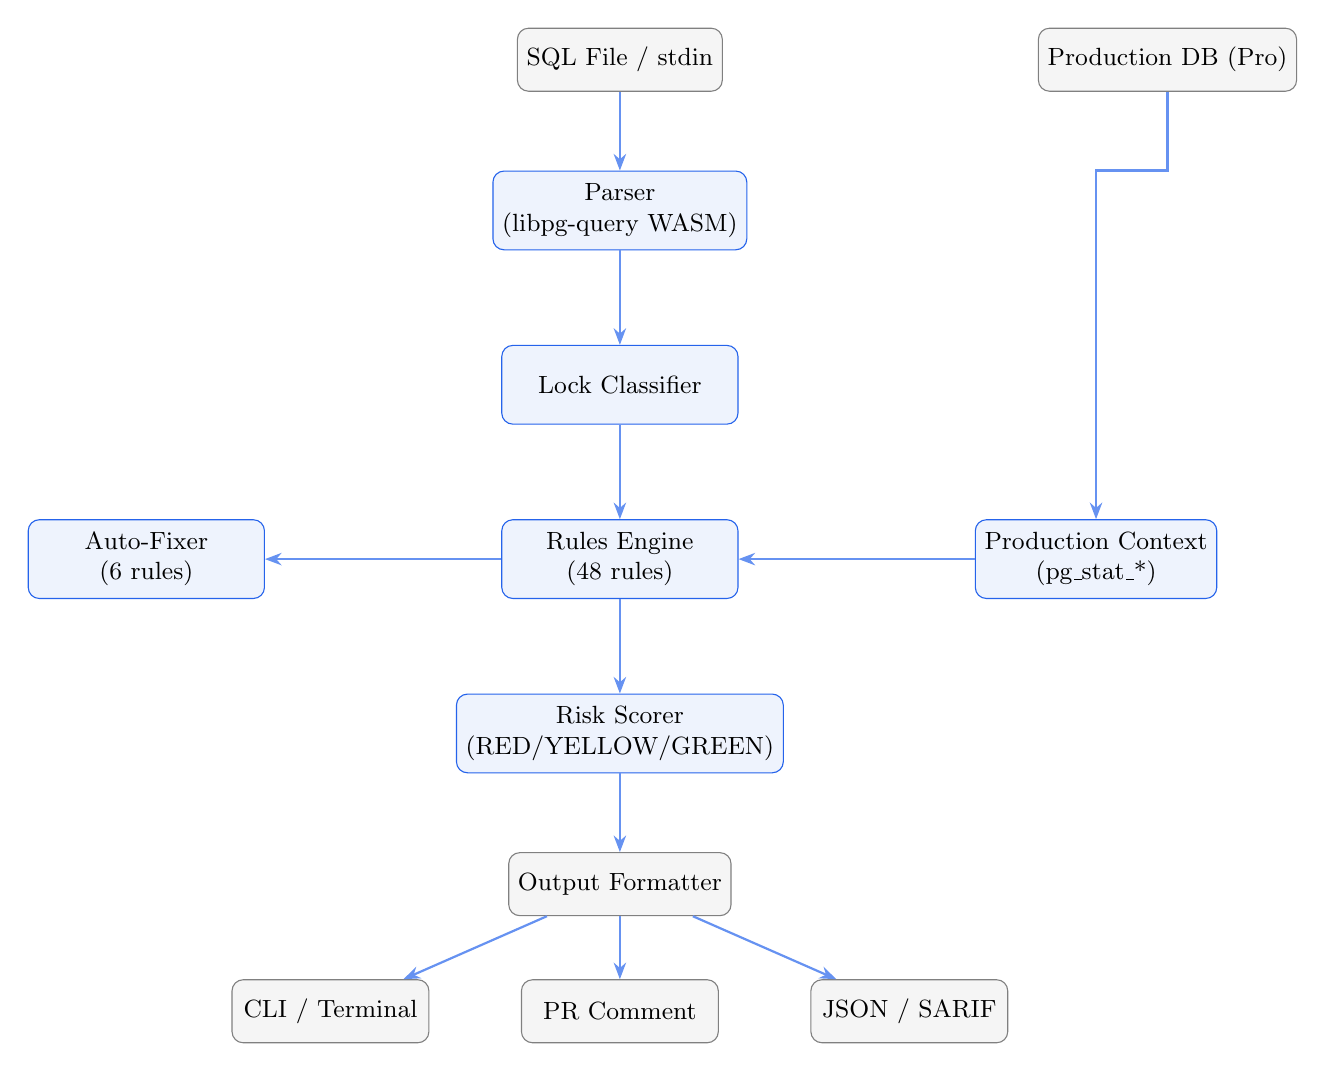
\begin{tikzpicture}[
  node distance=1.2cm and 2cm,
  block/.style={rectangle, draw=mpblue, fill=mpblue!8, rounded corners=4pt, minimum width=3cm, minimum height=1cm, align=center, font=\small},
  io/.style={rectangle, draw=gray, fill=gray!8, rounded corners=4pt, minimum width=2.5cm, minimum height=0.8cm, align=center, font=\small},
  arr/.style={-{Stealth[length=6pt]}, thick, color=mpblue!70},
]

% Input
\node[io] (sql) {SQL File / stdin};
\node[io, right=4cm of sql] (db) {Production DB (Pro)};

% Core pipeline
\node[block, below=1cm of sql] (parser) {Parser\\(libpg-query WASM)};
\node[block, below=of parser] (locks) {Lock Classifier};
\node[block, below=of locks] (rules) {Rules Engine\\(48 rules)};
\node[block, right=3cm of rules] (prod) {Production Context\\(pg\_stat\_*)};
\node[block, below=of rules] (scoring) {Risk Scorer\\(RED/YELLOW/GREEN)};
\node[block, left=3cm of rules] (fixer) {Auto-Fixer\\(6 rules)};

% Output
\node[io, below=1cm of scoring] (output) {Output Formatter};
\node[io, below left=0.8cm and 1cm of output] (cli) {CLI / Terminal};
\node[io, below=0.8cm of output] (pr) {PR Comment};
\node[io, below right=0.8cm and 1cm of output] (sarif) {JSON / SARIF};

% Arrows
\draw[arr] (sql) -- (parser);
\draw[arr] (db.south) -- ++(0,-1) -| (prod.north);
\draw[arr] (parser) -- (locks);
\draw[arr] (locks) -- (rules);
\draw[arr] (prod) -- (rules);
\draw[arr] (rules) -- (scoring);
\draw[arr] (rules) -- (fixer);
\draw[arr] (scoring) -- (output);
\draw[arr] (output) -- (cli);
\draw[arr] (output) -- (pr);
\draw[arr] (output) -- (sarif);

\end{tikzpicture}
\end{center}

\subsection{Module Breakdown}

\begin{tabularx}{\textwidth}{lX}
\toprule
\textbf{Module} & \textbf{Responsibility} \\
\midrule
\texttt{src/parser/} & DDL parsing with libpg-query WASM (real PostgreSQL parser compiled to WebAssembly) \\
\texttt{src/locks/} & Lock type classification --- pure lookup table mapping AST nodes to PG lock levels \\
\texttt{src/rules/} & 48 safety rules, engine, registry, shared helpers, inline disable comments \\
\texttt{src/production/} & Production context queries (Pro tier): pg\_stat\_*, pg\_class, pg\_stat\_statements \\
\texttt{src/scoring/} & Risk scoring engine: 0--100 scale based on lock severity, table size, query frequency \\
\texttt{src/fixer/} & Auto-fix engine for 6 rules (MP001, MP004, MP009, MP020, MP030, MP033) \\
\texttt{src/output/} & 6 formatters: text, JSON, SARIF v2.1.0, markdown, quiet, verbose, PR comment \\
\texttt{src/frameworks/} & Migration framework auto-detection (14 frameworks) \\
\texttt{src/config/} & Config file system + 3 built-in presets (recommended, strict, ci) \\
\texttt{src/analysis/} & Shared analyzeSQL pipeline, transaction boundaries, migration ordering \\
\texttt{src/generator/} & Safe migration SQL generation with lock\_timeout retry wrappers \\
\texttt{src/watch/} & File watcher with debounce for \texttt{watch} command \\
\texttt{src/hooks/} & Git pre-commit hook installer/uninstaller \\
\texttt{src/license/} & License key validation (HMAC-SHA256, client-side, no telemetry) \\
\texttt{src/billing/} & Stripe checkout + webhook + Resend email integration \\
\texttt{src/cli.ts} & CLI entry point (8 commands, commander.js) \\
\texttt{src/action/} & GitHub Action entry point \\
\texttt{src/index.ts} & Programmatic API (17 exports) \\
\bottomrule
\end{tabularx}

\subsection{Build Outputs}

\begin{tabularx}{\textwidth}{lllX}
\toprule
\textbf{Bundle} & \textbf{Size} & \textbf{Format} & \textbf{Purpose} \\
\midrule
CLI & 835 KB & CJS & \texttt{npx migrationpilot} / global install \\
Action & 1.2 MB & CJS & GitHub Action (single-file, no node\_modules) \\
API & 219 KB & ESM & Programmatic \texttt{import \{analyzeSQL\} from 'migrationpilot'} \\
\bottomrule
\end{tabularx}

\subsection{Test Coverage}

\begin{itemize}[nosep]
  \item \textbf{550+ tests} across \textbf{31 test files}
  \item Framework: Vitest + PGlite (in-process PostgreSQL for integration tests)
  \item Coverage areas: all 48 rules, CLI commands, output formats, config loading, auto-fix, framework detection, risk scoring, transaction analysis, migration ordering
  \item All tests pass with \texttt{pnpm test}, typecheck clean, lint clean
\end{itemize}

\newpage

% ══════════════════════════════════════════════════════════
% 7. CONFIGURATION
% ══════════════════════════════════════════════════════════

\section{Configuration}

\subsection{Config File}

Generated with \texttt{migrationpilot init}:

\begin{lstlisting}[style=yaml]
# .migrationpilotrc.yml
extends: migrationpilot:recommended

failOn: critical
pgVersion: 16

rules:
  MP037: false              # disable prefer-text-over-varchar
  MP004:
    severity: warning       # downgrade lock_timeout to warning
  MP011:
    severity: critical      # upgrade unbatched-backfill

exclude:
  - "migrations/legacy/**"
\end{lstlisting}

\subsection{Built-in Presets}

\begin{tabularx}{\textwidth}{lX}
\toprule
\textbf{Preset} & \textbf{Description} \\
\midrule
\texttt{migrationpilot:recommended} & Default severities, all rules enabled, fail on critical \\
\texttt{migrationpilot:strict} & All rules at critical severity, fail on warning \\
\texttt{migrationpilot:ci} & Optimized for CI: fail on critical, concise output \\
\bottomrule
\end{tabularx}

\subsection{Inline Disable Comments}

\begin{lstlisting}[style=sql]
-- migrationpilot-disable-next-line MP001
CREATE INDEX idx_users_email ON users (email);

-- migrationpilot-disable MP004, MP020
ALTER TABLE users ADD COLUMN bio TEXT;
-- migrationpilot-enable MP004, MP020
\end{lstlisting}

\newpage

% ══════════════════════════════════════════════════════════
% 8. POSTGRESQL LOCK REFERENCE
% ══════════════════════════════════════════════════════════

\section{PostgreSQL Lock Reference}

MigrationPilot classifies every DDL statement by the PostgreSQL lock level it acquires. This table shows the lock hierarchy from least to most restrictive:

\begin{tabularx}{\textwidth}{llccX}
\toprule
\textbf{Lock Level} & \textbf{Risk} & \textbf{Reads} & \textbf{Writes} & \textbf{Common Operations} \\
\midrule
ACCESS SHARE & \textcolor{mpgreen}{GREEN} & OK & OK & SELECT, ANALYZE \\
ROW SHARE & \textcolor{mpgreen}{GREEN} & OK & OK & SELECT FOR UPDATE \\
ROW EXCLUSIVE & \textcolor{mpgreen}{GREEN} & OK & OK & INSERT, UPDATE, DELETE \\
SHARE UPD EXCL & \textcolor{mpgreen}{GREEN} & OK & OK & CREATE INDEX CONCURRENTLY \\
SHARE & \textcolor{mpwarning}{YELLOW} & OK & \textcolor{mpcritical}{Blocked} & CREATE INDEX (non-concurrent) \\
SHARE ROW EXCL & \textcolor{mpwarning}{YELLOW} & OK & \textcolor{mpcritical}{Blocked} & CREATE TRIGGER \\
EXCLUSIVE & \textcolor{mpcritical}{RED} & OK & \textcolor{mpcritical}{Blocked} & REFRESH MATVIEW CONCURRENTLY \\
ACCESS EXCLUSIVE & \textcolor{mpcritical}{RED} & \textcolor{mpcritical}{Blocked} & \textcolor{mpcritical}{Blocked} & ALTER TABLE, DROP, VACUUM FULL \\
\bottomrule
\end{tabularx}

ACCESS EXCLUSIVE is the most dangerous --- it blocks \textbf{all} concurrent operations, including SELECT queries. MigrationPilot flags every statement that acquires this lock.

\newpage

% ══════════════════════════════════════════════════════════
% 9. COMMUNITY & PROJECT FILES
% ══════════════════════════════════════════════════════════

\section{Community \& Project Files}

MigrationPilot includes a complete set of community and project metadata files:

\begin{tabularx}{\textwidth}{lX}
\toprule
\textbf{File} & \textbf{Purpose} \\
\midrule
\texttt{README.md} & Comprehensive documentation with rules table, features, comparison, pricing \\
\texttt{LICENSE} & MIT License (Copyright 2026 Micke Samuel) \\
\texttt{CHANGELOG.md} & Version history with all changes \\
\texttt{CONTRIBUTING.md} & Contributor guide (setup, testing, rule development, PR process) \\
\texttt{CODE\_OF\_CONDUCT.md} & Contributor Covenant v2.1 \\
\texttt{SECURITY.md} & Security policy and vulnerability reporting \\
\texttt{.editorconfig} & Editor settings (2-space indent, LF, UTF-8) \\
\texttt{.env.example} & Environment variable template \\
\texttt{.github/FUNDING.yml} & GitHub Sponsors configuration \\
\texttt{.github/ISSUE\_TEMPLATE/} & Bug report and feature request templates \\
\texttt{.github/pull\_request\_template.md} & PR template with checklist \\
\texttt{.github/workflows/ci.yml} & CI pipeline (test, lint, typecheck, build) \\
\texttt{.github/workflows/publish.yml} & npm publish pipeline \\
\texttt{action.yml} & GitHub Action metadata \\
\texttt{docs/rules/*.md} & 48 per-rule documentation files (MP001--MP048) \\
\texttt{site/public/robots.txt} & SEO robots configuration \\
\texttt{site/public/sitemap.xml} & 49-URL sitemap (homepage + 48 rule pages) \\
\bottomrule
\end{tabularx}

\newpage

% ══════════════════════════════════════════════════════════
% 10. SEO & METADATA
% ══════════════════════════════════════════════════════════

\section{SEO \& Metadata}

\subsection{Open Graph / Social Sharing}

The site generates a dynamic Open Graph image at build time using Next.js edge runtime:

\begin{itemize}[nosep]
  \item \textbf{Size:} 1200$\times$630 pixels (standard OG)
  \item \textbf{Content:} MP logo, ``MigrationPilot'' title, tagline, 4 feature pills, domain
  \item \textbf{Twitter card:} summary\_large\_image
\end{itemize}

\subsection{HTML Metadata}

\begin{lstlisting}[style=terminal]
<title>MigrationPilot -- PostgreSQL Migration Safety</title>
<meta name="description" content="Know exactly what your
  PostgreSQL migration will do to production -- before you
  merge. 48 safety rules, auto-fix, risk scoring..." />
<meta name="keywords" content="postgresql, migration,
  database, safety, DDL, locks, github action, CLI,
  linter, static analysis, zero downtime" />
<link rel="canonical" href="https://migrationpilot.dev" />
<meta property="og:image"
  content="https://migrationpilot.dev/opengraph-image" />
\end{lstlisting}

\subsection{npm Package Metadata}

\begin{lstlisting}[style=json]
{
  "name": "migrationpilot",
  "version": "1.1.0",
  "description": "PostgreSQL migration safety CLI...",
  "keywords": ["postgresql", "migration", "database",
    "safety", "linter", "github-action", "ddl", "sql",
    "static-analysis", "zero-downtime", "lock", "pg"],
  "bugs": {
    "url": "https://github.com/mickelsamuel/migrationpilot/issues"
  },
  "funding": {
    "type": "github",
    "url": "https://github.com/sponsors/mickelsamuel"
  }
}
\end{lstlisting}

\vfill

\begin{center}

\begin{tikzpicture}
  \node[fill=mpblue, rounded corners=6pt, minimum width=1.2cm, minimum height=1.2cm, text=white, font=\large\bfseries] {MP};
\end{tikzpicture}

\vspace{0.5cm}
{\large\bfseries MigrationPilot v1.1.0}\\[0.2cm]
{\color{gray} Know exactly what your PostgreSQL migration will do to production.}\\[0.5cm]
{\small
\url{https://migrationpilot.dev} $\cdot$
\url{https://github.com/mickelsamuel/migrationpilot} $\cdot$
\texttt{npm install migrationpilot}
}
\end{center}

\end{document}
